\pr (2b) Vyberte funkciu, ktorej definičný obor je znázornený na obrázku.

\begin{multicols}{2}
\noindent
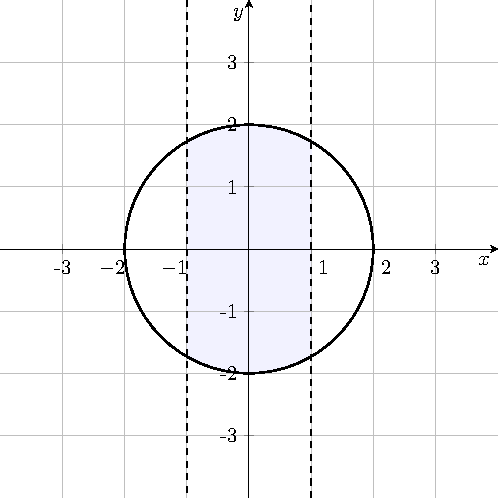
\includegraphics{kruznica1.pdf}

\noindent
\begin{itemize}
\item[a)] $\displaystyle f(x,y)= \sqrt{x}+\ln{(4-x^2-y^2)}$
\item[b)] $\displaystyle f(x,y)= \arcsin x+\sqrt{4-x^2-y^2}$ % OK
\item[c)] $\displaystyle f(x,y)= \frac{\ln(x+1)}{\sqrt{4-x^2-y^2}}$
\item[d)] $\displaystyle f(x,y)= \frac{\arcsin{(x+y)}}{\sqrt{4-x^2-y^2}}$
\end{itemize}
\end{multicols}
